\section{Extended Counterfactual Stratification and Zero-VLM Risk-Gate Diagnostics}
\label{app:mechanisms_risk}

\begin{table*}[!t]
\centering
\caption{Side-by-side dual-family pixel-exact counterfactual evaluation across \textsc{Qwen3-VL-8B} ($1{,}440$ evaluations) and \textsc{InternVL3.5-8B-HF} ($1{,}440$ evaluations), spanning factorial contrasts ($480$ all vs.\ $473$ bit-identical mask subset, $\mathrm{IoU}{=}1.000$), prior optical regimes, and objective pixel-distortion groupings.}
\label{tab:app-counterfactual-dual}
\resizebox{\textwidth}{!}{% Generated automatically by build_cviu_appendix_assets.py from optical_mechanisms.json
\begin{tabular}{@{}lrrrr@{}}
\toprule
Subgroup / Counterfactual Contrast & Pairs ($n$) & Metric & \textsc{Qwen3-VL-8B} (\% / 95\% CI) & \textsc{InternVL3.5-8B-HF} (\% / 95\% CI) \\
\midrule
\multicolumn{5}{@{}l}{\textit{Panel A: Factorial Counterfactual Contrast (All 480 Pairs vs.\ Exact-Mask 473 Subset, $\mathrm{IoU}=1.000$)}} \\
Photometric Matched ($I^{\text{photo}}$ vs.\ $I^O$) & 480 & Flip\% & 5.83 [3.75, 8.12] & 7.08 [5.00, 9.38] \\
Background Swap Only ($I^B$ vs.\ $I^O$) & 480 & Flip\% & 6.46 [4.58, 8.54] & 9.17 [6.67, 11.88] \\
Target Silhouette Only ($I^T$ vs.\ $I^O$) & 480 & Flip\% & 8.12 [5.62, 10.83] & 9.79 [7.29, 12.50] \\
Full Conversion ($I^F$ vs.\ $I^O$) & 480 & Flip\% & 9.38 [7.08, 11.67] & 10.62 [7.92, 13.54] \\
Non-Photometric Residual ($I^F - I^{\text{photo}}$) & 480 & $\Delta$Flip & +3.54 [+1.25, +5.83] & +3.54 [+1.04, +6.04] \\
Exact-Mask Residual ($\mathrm{IoU}=1.000$, $n{=}473$) & 473 & $\Delta$Flip & +3.38 [+1.26, +5.70] & +3.38 [+0.84, +5.97] \\
\midrule
\multicolumn{5}{@{}l}{\textit{Panel B: Prior Surface Optical Regimes ($\Delta H = H_C - H_O$ and Flip Rate)}} \\
Reflective/Metallic & 158 & $\Delta H$ (Flip) & +4.43\% (10.76\%) & +0.63\% (10.76\%) \\
Emissive/Screen & 58 & $\Delta H$ (Flip) & +0.00\% (3.45\%) & +6.90\% (13.79\%) \\
Transparent/Glass & 176 & $\Delta H$ (Flip) & +0.57\% (9.66\%) & +1.70\% (9.66\%) \\
Matte/Diffuse & 88 & $\Delta H$ (Flip) & +1.14\% (10.23\%) & -1.14\% (10.23\%) \\
\midrule
\multicolumn{5}{@{}l}{\textit{Panel C: Objective Pixel-Distortion Regimes (Independent of Category Labels)}} \\
Low-Distortion & 133 & $\Delta H$ (Flip) & +3.76\% (6.77\%) & +3.01\% (10.53\%) \\
Texture/Detail-Degraded & 327 & $\Delta H$ (Flip) & +0.92\% (10.09\%) & +0.61\% (10.40\%) \\
Specular-Stripped & 14 & $\Delta H$ (Flip) & -7.14\% (7.14\%) & +0.00\% (14.29\%) \\
Mask/Opacity-Shift & 6 & $\Delta H$ (Flip) & +33.33\% (33.33\%) & +16.67\% (16.67\%) \\
\bottomrule
\end{tabular}
}
\end{table*}

\begin{figure*}[!t]
\centering
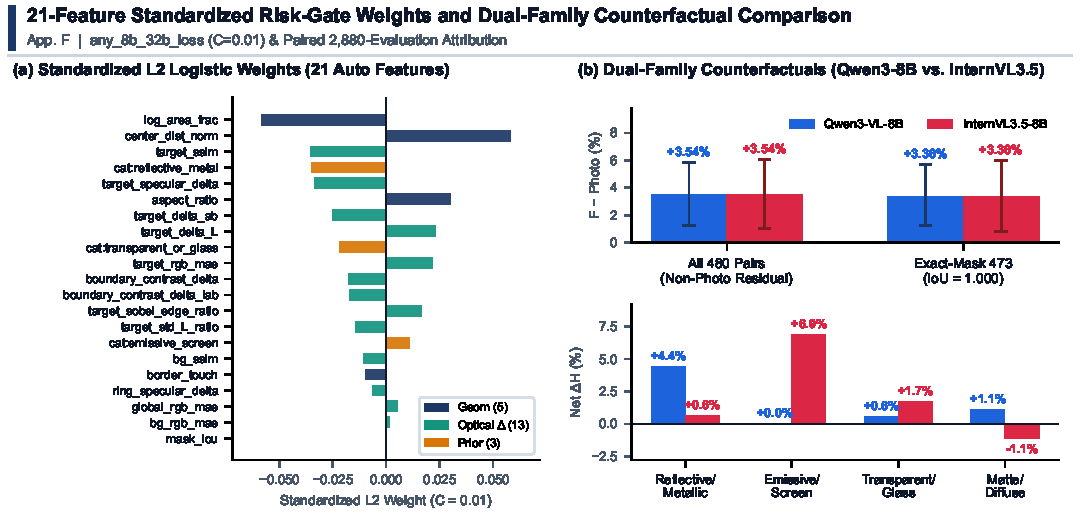
\includegraphics[width=0.97\textwidth]{app_fig5_features_and_counterfactuals.pdf}
\caption{\textbf{Full 21-feature standardized risk-gate coefficients and dual-family counterfactual residual invariance.}
\emph{(a)} Standardized $\ell_2$ logistic regression weights ($C{=}0.01$) predicting family-calibrated \textsc{Qwen3-VL} regressions (\texttt{any\_8b\_32b\_loss}), separated into simulator mask geometry (5 cues), paired appearance/edge deltas (13 cues), and coarse category priors (3 cues).
\emph{(b)} Side-by-side comparison across \textsc{Qwen3-VL-8B} and \textsc{InternVL3.5-8B-HF}: identical $+3.54\%$ ($+3.38\%$ on bit-identical masks) non-photometric \textsc{BSDF} residual above $\mathrm{CIE}~L^*a^*b^*$ matching alongside diverging regime gains.}
\label{fig:app-features-cf}
\end{figure*}

\subsection{Cross-family counterfactual invariance and mask-support sensitivity}
Table~\ref{tab:app-counterfactual-dual} and Figure~\ref{fig:app-features-cf}(b) expand Section~\ref{sec:mechanisms} with full confidence intervals across all $2{,}880$ counterfactual evaluations (\textsc{Qwen3-VL-8B} and \textsc{InternVL3.5-8B-HF}). Although \textsc{InternVL3.5-8B-HF} starts from slightly higher baseline photometric sensitivity ($7.08\%$ vs.\ $5.83\%$ flip rate on $I^{\text{photo}}$) and full conversion turnover ($10.62\%$ vs.\ $9.38\%$), subtracting the $\mathrm{CIE}~L^*a^*b^*$-matched luminance/chromatic control reveals an identical \textbf{$+3.54\%$ non-photometric shader residual} ($[+1.25\%, +5.83\%]$ and $[+1.04\%, +6.04\%]$). Restricting the comparison to the $473/480$ pairs with bit-identical simulator masks ($\mathrm{IoU}{=}1.000$) yields virtually unchanged residuals of \textbf{$+3.38\%$} on both architectures ($[+1.26\%, +5.70\%]$ and $[+0.84\%, +5.97\%]$), confirming that silhouette boundary anti-aliasing on the remaining $7$ pairs does not confound the optical finding. Under objective pixel-distortion grouping (Panel~C), \emph{Low-Distortion} targets gain $+3.76\%$ (\textsc{Qwen3}) and $+3.01\%$ (\textsc{InternVL3.5}), whereas heavily \emph{Specular-Stripped} targets suffer $-7.14\%$ net drop on \textsc{Qwen3-VL-8B}.

\begin{table*}[!t]
\centering
\caption{Complete 21-feature zero-\textsc{VLM} risk-gate inventory (\texttt{deploy\_auto}), reporting group membership, mean $\pm$ SD stratified by \textsc{Qwen3-VL} regression status (\texttt{any\_8b\_32b\_loss}: $455$ non-loss vs.\ $25$ loss pairs), direction-aligned univariate \textsc{AUROC}, and fitted standardized $\ell_2$ weights ($C{=}0.01$).}
\label{tab:app-features21}
\resizebox{\textwidth}{!}{% Generated automatically by build_cviu_appendix_assets.py from pair_optical_features.json & risk_auditor.json
\begin{tabular}{@{}llrrrr@{}}
\toprule
Feature Name & Definition & No-Loss ($n{=}455$) & Loss ($n{=}25$) & Univar.\ AUROC & $\ell_2$ Weight $w_j$ \\
\midrule
\multicolumn{6}{@{}l}{\textit{Simulator Mask Geometry (5)}} \\
\texttt{log\_area\_frac} & Logarithm of target pixel area fraction & -2.432 $\pm$ 0.921 & -2.888 $\pm$ 0.890 & 0.665 & -0.0585 \\
\texttt{aspect\_ratio} & Target bounding-box width-to-height ratio & 1.270 $\pm$ 1.122 & 1.561 $\pm$ 1.194 & 0.560 & +0.0303 \\
\texttt{center\_dist\_norm} & Euclidean distance from frame center (normalized) & 0.331 $\pm$ 0.058 & 0.378 $\pm$ 0.063 & 0.703 & +0.0584 \\
\texttt{border\_touch} & Indicator whether target bbox touches image border & 0.020 $\pm$ 0.139 & 0.000 $\pm$ 0.000 & 0.510 & -0.0097 \\
\texttt{mask\_iou} & Mask overlap IoU between original and converted captures & 0.998 $\pm$ 0.026 & 1.000 $\pm$ 0.000 & 0.508 & +0.0000 \\
\midrule
\multicolumn{6}{@{}l}{\textit{Paired Optical, Chromatic \& Structural Deltas (13)}} \\
\texttt{global\_rgb\_mae} & Full-frame mean absolute RGB difference & 0.110 $\pm$ 0.048 & 0.120 $\pm$ 0.072 & 0.510 & +0.0053 \\
\texttt{target\_rgb\_mae} & Target-mask mean absolute RGB difference & 0.126 $\pm$ 0.094 & 0.193 $\pm$ 0.180 & 0.577 & +0.0216 \\
\texttt{bg\_rgb\_mae} & Background mean absolute RGB difference & 0.108 $\pm$ 0.047 & 0.114 $\pm$ 0.076 & 0.549 & +0.0017 \\
\texttt{target\_delta\_L} & Mean target lightness shift $|\Delta L^*|$ & 8.866 $\pm$ 9.387 & 16.134 $\pm$ 19.356 & 0.566 & +0.0229 \\
\texttt{target\_delta\_ab} & Mean target chromatic shift $\|\Delta(a^*, b^*)\|_2$ & 1.122 $\pm$ 1.742 & 0.801 $\pm$ 1.142 & 0.568 & -0.0248 \\
\texttt{target\_std\_L\_ratio} & Converted-to-original lightness std ratio on target & 1.048 $\pm$ 0.573 & 1.055 $\pm$ 0.428 & 0.515 & -0.0142 \\
\texttt{target\_ssim} & Local $8{\times}8$ structural similarity inside target & 0.652 $\pm$ 0.207 & 0.560 $\pm$ 0.221 & 0.618 & -0.0353 \\
\texttt{bg\_ssim} & Local $8{\times}8$ structural similarity on background & 0.762 $\pm$ 0.120 & 0.763 $\pm$ 0.122 & 0.506 & -0.0104 \\
\texttt{target\_sobel\_edge\_ratio} & Converted-to-original Sobel $|\nabla L^*|$ ratio on target & 0.957 $\pm$ 0.775 & 0.941 $\pm$ 0.430 & 0.505 & +0.0164 \\
\texttt{target\_specular\_delta} & Highlight pixel ($Y>0.88$) fraction shift on target & 0.008 $\pm$ 0.086 & -0.013 $\pm$ 0.193 & 0.514 & -0.0333 \\
\texttt{ring\_specular\_delta} & 12-px exterior ring specular fraction shift & 0.001 $\pm$ 0.034 & 0.014 $\pm$ 0.056 & 0.558 & -0.0063 \\
\texttt{boundary\_contrast\_delta} & 8-px inner/outer contour lightness contrast shift & -0.445 $\pm$ 8.405 & -5.479 $\pm$ 13.232 & 0.623 & -0.0176 \\
\texttt{boundary\_contrast\_delta\_lab} & 8-px inner/outer contour $\mathrm{CIE}~\Delta E_{ab}^*$ shift & -0.621 $\pm$ 8.225 & -5.452 $\pm$ 13.202 & 0.615 & -0.0169 \\
\midrule
\multicolumn{6}{@{}l}{\textit{Coarse Target Category Priors (3)}} \\
\texttt{cat\_is\_transparent\_or\_glass} & Transparent/glass object category prior & 0.070 $\pm$ 0.256 & 0.000 $\pm$ 0.000 & 0.535 & -0.0220 \\
\texttt{cat\_is\_reflective\_appliance\_or\_metal} & Reflective appliance/metal category prior & 0.402 $\pm$ 0.490 & 0.440 $\pm$ 0.496 & 0.519 & -0.0348 \\
\texttt{cat\_is\_emissive\_or\_screen} & Emissive/screen category prior & 0.185 $\pm$ 0.388 & 0.160 $\pm$ 0.367 & 0.512 & +0.0109 \\
\bottomrule
\end{tabular}
}
\end{table*}

\subsection{Per-feature breakdown of the 21-cue zero-VLM risk gate}
Table~\ref{tab:app-features21} and Figure~\ref{fig:app-features-cf}(a) dissect why lightweight pre-deployment risk gating achieves $0.743$ test \textsc{AUROC} ($0.732$ 30-scene \textsc{LOSO} with \texttt{geometry\_only}, catching $52.0\%$ of regressions in the top $20\%$ triage budget) while global \textsc{RGB MAE} fails ($0.432$ test \textsc{AUROC}). Regression targets are systematically smaller (\texttt{log\_area\_frac}: $-2.888$ vs.\ $-2.432$, weight $-0.0585$), positioned closer to frame peripheries (\texttt{center\_dist\_norm}: $0.378$ vs.\ $0.331$, univariate \textsc{AUROC} $= 0.703$, weight $+0.0584$), and undergo stronger local structural degradation inside the target mask (\texttt{target\_ssim}: $0.560$ vs.\ $0.652$, weight $-0.0353$) alongside negative boundary contrast shifts (\texttt{boundary\_contrast\_delta}: $-5.479$ vs.\ $-0.445$, univariate \textsc{AUROC} $= 0.623$). By contrast, \texttt{global\_rgb\_mae} carries near-random univariate separability ($0.510$) because global metallic reflections inflate pixel differences on easy scenes where glare removal improves grounding.
